\documentclass{recipe}

\begin{document}
\begin{recipe}{Tomato Soup with Grilled Cheese}
  \servings{1}

  \begin{ingredients}
    \ingredient{1}{tbsp}{butter}
    \ingredient{4}{slices}{white sandwich bread}
    \ingredient{2}{slices}{american cheese}
    \ingredient{10.75}{oz}{condensed tomato soup}
    \ingredient{5}{oz}{milk}
    \ingredient{}{}{garlic powder}
    \ingredient{}{}{dry basil}
    \ingredient{}{}{red pepper flakes}
  \end{ingredients}

  \begin{images}
    \begin{image}
      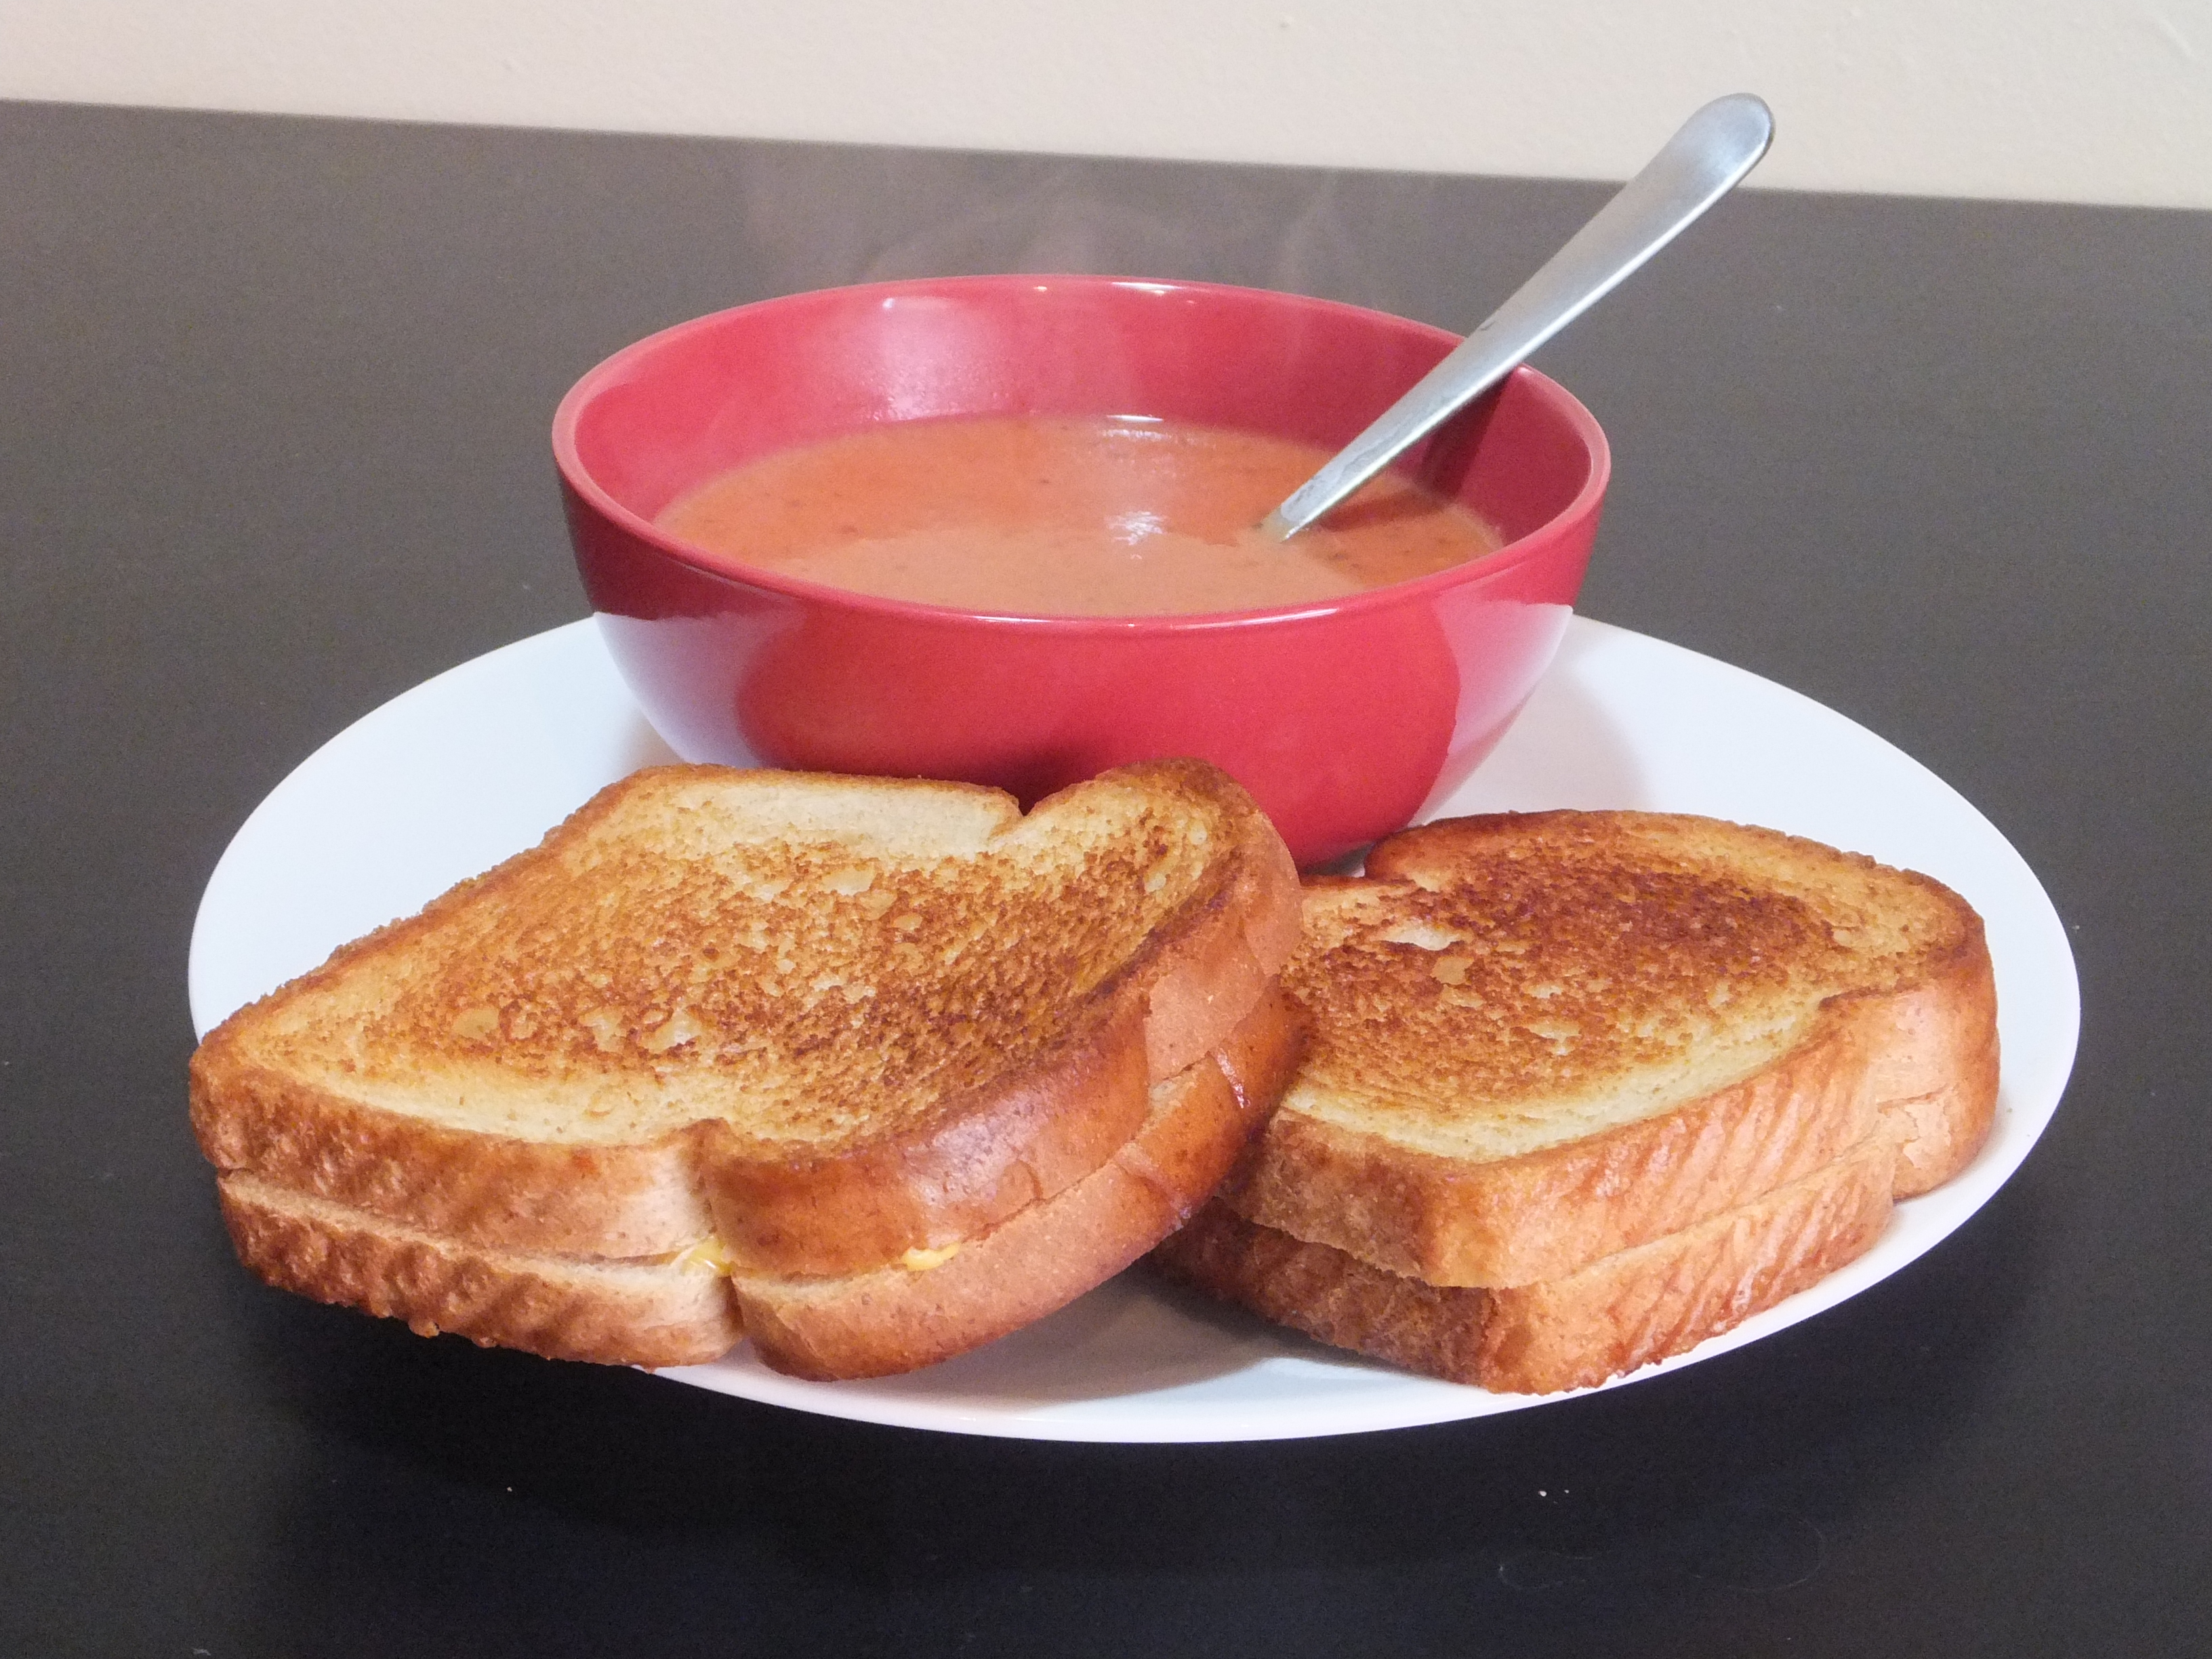
\includegraphics[width=0.9\linewidth]{grilled_cheese_tomato-01.jpeg}
    \end{image}
  \end{images}

  \begin{steps}
  \item Set your griddle to 350\degree F, or about medium-low on a
    range.
  \item Put a sauce pan on medium-low heat and add the tomato soup
    concentrate along with all the spices.
  \item Thoroughly mix the spices into the soup and heat the soup
    until just bubbling a bit.  Make sure to stir it regularly, as
    it'll be pretty thick at this point and won't heat well.
  \item When the griddle heats, spray it with oil, divide the butter
    in four, and add two chunks to the griddle.  Swirl the butter
    around to make an even layer.
  \item Put the bread and cheese on top of the pools of butter on the
    griddle.
  \item Cook the bread on one side until it's brown, trying not to
    move it if possible.
  \item Re-butter the griddle and flip the sandwiches.
  \item Add the milk to the soup mixture and mix well
  \item Wait for the grilled cheese to finish and serve it with the
    soup.  It's usually best to take the soup off a bit early as
    otherwise it'll be too hot (though a bunch of cold milk just went
    in, so you need it to heat some).
  \end{steps}
\end{recipe}
\end{document}
